\documentclass[a4paper, 11pt]{article}
\usepackage[utf8]{inputenc}
\usepackage[brazil]{babel}
\usepackage[dvipdfm, a4paper, top=1in, left=1in, right=1in]{geometry}
\usepackage{hyperref}
\usepackage{multicol}
\usepackage{amsmath}
\usepackage{graphicx}
\begin{document}
\title{Trabalho Pratico II - Compressor de Arquivos}
\author{Joao Paulo Mendes de Sa}
\date{}
\maketitle
\section{Introdução}
O algorítimo de Huffman é capaz de gerar um código de tamanho variável para um conjunto de símbolos com a finalidade de otimizar a quantidade de bits necessárias para armazenar o conteúdo de um arquivo. Códigos menores são usados para representar símbolos que ocorrem no arquivo com mais frequência e os maiores para símbolos com menor frequência. O algorítimo de Huffman gera uma arvore binaria onde o caminho ate cada folha é o seu código. Dessa maneira é impossível gerar um código que seja o prefixo de outro código na mesma arvore pois apenas folhas guardam símbolos. Os passos básicos do algoritmo de Huffman para gerar a arvore sabendo a frequência de cada simbolo são:
\begin{enumerate}
\item Crie uma fila de prioridades com nodos de uma arvore onde os items de menor frequência tendo maior prioridade.
\item Enquanto ha mais de um nodo na fila:
\begin{enumerate}
\item Remova os dois primeiros nodos da fila
\item Crie um novo nodo e faca a sua esquerda e direita apontar para os dois nodos retirados
\item A frequência desse nodo é igual a soma das frequências dos nodos retirados
\item Insira esse nodo de novo na fila
\end{enumerate}
\item O nodo que resta é a raiz da arvore
\end{enumerate}
Para determinar o código para um simbolo basta navegar da raiz ate o nodo que contem o simbolo. Cada esquerda é um 0 e cada direita é um 1. A distancia de uma folha ate a raiz é o tamanho do código gerado.

\section{Implementação}
\subsection{Estrutura de Dados}
Foi criado um tipo abstrato de dados para manipular o heap, um para gerar a arvore de Huffman, e outro para comprimir e descomprimir o arquivo dado uma arvore contendo a codificação.

O heap armazenava todas as folhas na arvore e contia informações sobre o simbolo original, a frequência que ele aparecia, o tamanho do código gerado pelo algoritmo de Huffman, o código gerado, e ponteiros para outras folhas. A arvore era composto desses mesmos subitens do heap mais um ponteiro adicional para a raiz da arvore.

Para implementar a fila de prioridade foram usados dois heaps ao invés de uma lista encadeada. Dessa maneira o algorítimo é muito mais eficiente. Com apenas uma lista ordenada remoção seria $O(1)$ pois bastaria fazer a cabeça da lista apontar para o próximo, inserção seria $O(n)$ pois seria necessário buscar pela lista inteira ate achar o lugar de inserção, e ordenação $O(n^2)$ através de seleção ou inserção. Usando dois heaps remoção virou $O(log(n))$ logo que a função heapify() mantem as propriedades de uma heap navegando ele como uma arvore binaria, inserção $O(1)$ pois como a soma de dois nodos sempre seria maior que todos nodos anteriores bastava reinserir o nodo na ultima posição do segundo heap, e ordenação $O(nlog(n))$ usando heapsort.

\subsection{Funções e Procedimentos}
\begin{verbatim}
unsigned long file_len(FILE* file);
\end{verbatim} 
Recebe um arquivo e retorna o seu tamanho em bits.

\begin{verbatim}
void heap_init(heap_t *heap);
\end{verbatim} 
Aloca memoria para armazenar os símbolos no heap e inicializa todos eles.

\begin{verbatim}
void heap_dealloc(heap_t *heap);
\end{verbatim} 
Libera a memoria alocada ao heap.

\begin{verbatim}
void heap_fill(heap_t *heap, FILE *file);
\end{verbatim} 
Ler um arquivo e determina a frequência de cada simbolo no arquivo

\begin{verbatim}
void heap_condense(heap_t *heap);
\end{verbatim} 
Apos o heap\_fill() essa função remove do vetor do heap os items que tem frequência igual a 0 e determina o numero de símbolos diferentes que apareceram

\begin{verbatim}
int heapCmp_freq(byte_t a, byte_t b);
int heapCmp_symb(byte_t a, byte_t b);
\end{verbatim} 
Ambas usados com ponteiros para funções pelas funções que mantem o heap. A primeira ordena por frequência do simbolo e a segunda por ordem alphabetic do simbolo.

\begin{verbatim}
void heapify(heap_t *heap, int father, int (*cmp)(byte_t, byte_t));
\end{verbatim} 
Função navega o vetor do heap como uma arvore e verifica se o heap ainda é um heap. Se não o concerta.

\begin{verbatim}
void heap_build(heap_t *heap, int (*cmp)(byte_t, byte_t));
\end{verbatim} 
Cria um heap a partir de um vetor ordenado. O critério e decido por uma outra função passada por ponteiro.

\begin{verbatim}
void heap_sort(heap_t *heap, int (*cmp)(byte_t, byte_t));
\end{verbatim} 
Ordena um vetor usando heapsort e o critério dado pela função. Primeiro cria um heap do vetor com heap\_build() e depois remove primeiro item e o coloca na ultima posição do vetor. Conserta o heap com heapify() e repete ate o vetor estar ordenado.

\begin{verbatim}
void heap_clone(heap_t original, heap_t* clone);
\end{verbatim} 
Duplica um heap.

\begin{verbatim}
byte_t heap_extract_min(heap_t *heap, int(*cmp)(byte_t, byte_t));
\end{verbatim} 
Remove of menor item to heap e chama heapify() para consertar depois.

\begin{verbatim}
byte_t* huff_build_tree(heap_t huffQueue);
\end{verbatim} 
Implementa o algorítimo de Huffman. Duplica o heap e cria um heap auxiliar. Enquanto houver mais de um elemento entre os dois heap remove os dois com menores frequências e cria uma subárvore e o reinsere no fim do segundo heap. Retorna a raiz para a arvore gerada.

\begin{verbatim}
void tree_dealloc(byte_t *node);
\end{verbatim} 
Faz um caminhamento preordem da arvore e desaloca a memoria usada por cada nodo.

\begin{verbatim}
int bsearchCmp_symb(const void* a, const void* b);
\end{verbatim} 
Usada por bsearch() como critério para buscar um simbolo.

\begin{verbatim}
void bin_to_dec(char* binary, unsigned short *dec, short bits);
\end{verbatim} 
Pega um numero binário representado por uma string (little endian) e converte para base 10

\begin{verbatim}
void huff_build_decode_table(heap_t *heap, tree_t tree);
\end{verbatim} 
Navega arvore de Huffman e determina o código usado para representar cada simbolo. Escreve essa informação no heap.

\begin{verbatim}
void file_write_header(FILE *outputFile, heap_t heap, 
                       unsigned long inputFileLen);
\end{verbatim} 
Escreve of cabeçalho no inicio do arquivo a ser comprimido.

\begin{verbatim}
%void dec_to_bin(unsigned short dec, char* prefixBin, short bits);
\end{verbatim} 
Faz of inverso de bin\_to\_dec().

\begin{verbatim}
void write_bit(FILE *outputFile, short prefix, short prefixLen);
\end{verbatim} 
Usando bitmasking escreve cada bit do código de Huffman de um simbolo a um buffer. Quando o buffer é preenchido por oito bits escreve o byte no arquivo.

\begin{verbatim}
void file_compress(FILE *outputFile, FILE *inputFile, heap_t heap, 
                   unsigned long inputFileLen);
\end{verbatim} 
Efetua a compressão. Ler o arquivo a ser comprimido e produz um bitstream usando write\_bit() para escrever no arquivo a ser comprimido.

\begin{verbatim}
unsigned long file_parse_header(FILE *compressedFile, tree_t *huff);
\end{verbatim} 
Ler o cabeçalho de um arquivo e reconstrói a arvore de Huffman. Começa por um nodo raiz e vai navegando pelo código de Huffman de cada character. Se um nodo não existe então a função aloca espaço para ele ate chegar na folha correta. Repete isso para todos símbolos.

\begin{verbatim}
void file_decompress(FILE *compressedFile, FILE *outputFile, tree_t huff, 
                     unsigned long fileLen);
\end{verbatim} 
Efetua a descompressão do bitstream. Usando a arvore reconstituída ele lé um byte e escreve no buffer. Esse buffer e convertido para um numero binário e o caminhamento da arvore é feito ate encontrar uma folha. O simbolo decodificado e escrito no arquivo. Isso repete ate o buffer esvaziar. Quando vazio ele lé outro bit ate o arquivo descomprimido esteja do seu tamanho original.

\subsection{Programa Principal}
é necessário ler o arquivo a ser comprimido duas vezes. Uma para determinar os símbolos que aparecem que nessa caso foi cada byte e a frequência na qual ele ocorre.
A segunda leitura é a que realmente comprime o arquivo usando o código gerado pelo algorítimo de Huffman. Primeiro é escrito um cabeçalho no arquivo comprimido comas informações necessárias para decodificá-lo e finalmente o conteúdo do arquivo a ser comprimido se transforma no bitstream codificado que é escrito no arquivo comprimido. Para descomprimir o arquivo bastava apenas reconstruir a arvore. Um processo simples sendo que todas informações necessárias estão presente no cabeçalho.

\subsection{Organização do Código, Decisões de Implementação e Detalhes Técnicos}
O código esta divido em quatro arquivos. huff.c e huff.h contem todas a funções necessárias para efetuar a compressão e descompressão de um arquivo. comprima.c contem o procedimento para comprimir um arquivo e descomprima.c faz o inverso. Para significar a implementação do algorítimo o maior codigo de huffman que o programa é capaz de gerar é de 64 bits pela limitação que o maior tipo em ANSI C90 é unsigned long long isso é menor que o limite teórico de 256 bits. Para retificar essa limitação eu podia separar o código de um simbolo em 4 variáveis que daria 256 bits no total. Mas essa alteração aumentaria a complexidade do código significadamente. Para verificar se esse limite era encontrado em casos reais eu gerei 10 arquivos com conteúdos randômicos entre 100MB e 1GB e nunca encontrei um caso onde essa limitação ficou aparente.

O formato usado no cabeçalho de decodificação foi:
\begin{center}
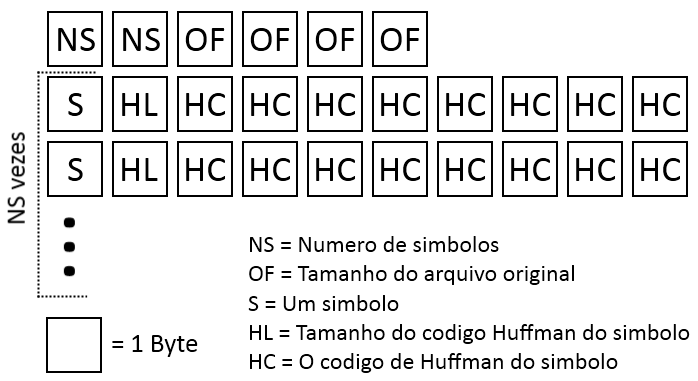
\includegraphics[width=4in]{header.png}
\end{center}

O compilador usado foi gcc 4.6.020110429 no sistema operacional Arch Linux 2.6.38-ARCH. Para executar o compressor basta digitar na linha de commando ./comprima FILEOUT FILEIN e para o descompressor ./descomprima FILEOUT FILEIN.

\section{Analise de Complexidade}
A variável $x$ é definido como o tamanho do arquivo em bits. A variável $n$ é definido como o numero de símbolos diferentes (no máximo 256).

\begin{verbatim}
unsigned long file_len(FILE* file);
\end{verbatim} 
Não depende da entrada logo determina o tamanho em $O(1)$.

\begin{verbatim}
void heap_init(heap_t *heap);
\end{verbatim} 
Não depende da entrada longo aloca e inicializa em $O(1)$.

\begin{verbatim}
void heap_dealloc(heap_t *heap);
\end{verbatim} 
Não depende da entrada long desaloca em $O(1)$.

\begin{verbatim}
void heap_fill(heap_t *heap, FILE *file);
\end{verbatim} 
Para cada byte do arquivo incrementa a frequência de um simbolo no heap logo $O(x)$.

\begin{verbatim}
void heap_condense(heap_t *heap);
\end{verbatim} 
Os dois loops aninhados tem tamanho fixo logo não depende da entrada então $O(1)$.

\begin{verbatim}
int heapCmp_freq(byte_t a, byte_t b);
int heapCmp_symb(byte_t a, byte_t b);
\end{verbatim} 
Cada um faz apenas uma comparação independente do tamanho logo $O(1)$.

\begin{verbatim}
void heapify(heap_t *heap, int father, int (*cmp)(byte_t, byte_t));
\end{verbatim} 
Navega um vetor como uma arvore, no pior caso navega de uma raiz ate uma folha que é $O(log(n))$.

\begin{verbatim}
void heap_build(heap_t *heap, int (*cmp)(byte_t, byte_t));
\end{verbatim} 
Chama heapify() para cada metade de n longo $O(nlog(n))$.

\begin{verbatim}
void heap_sort(heap_t *heap, int (*cmp)(byte_t, byte_t));
\end{verbatim} 
Constrói o heap com heap\_build() e depois para cada n a função remove a raiz do heap e reinsere na ultima posição do vetor. $max(O(nlog(n)), O(nlog(n))) = O(nlog(n))$.

\begin{verbatim}
void heap_clone(heap_t original, heap_t* clone);
\end{verbatim} 
Um loop depende no numero de símbolos logo $O(n)$.

\begin{verbatim}
byte_t heap_extract_min(heap_t *heap, int(*cmp)(byte_t, byte_t));
\end{verbatim} 
Chama heapify() uma vez então $O(log(n))$.

\begin{verbatim}
byte_t* huff_build_tree(heap_t huffQueue);
\end{verbatim} 
Um loop para inicializar um heap auxiliar O(n). Um loop para o algorítimo de Huffman que também executa n vezes e chama heap\_extract\_min() duas vezes logo é $2O(n)O(log(n)) = O(nlog(n))$.

\begin{verbatim}
void tree_dealloc(byte_t *node);
\end{verbatim} 
Navega todos os nodos da arvore que são no máximo $2n - 1$ logo $O(n)$.

\begin{verbatim}
int bsearchCmp_symb(const void* a, const void* b);
\end{verbatim} 
Uma comparação $O(1)$.

\begin{verbatim}
void bin_to_dec(char* binary, unsigned short *dec, short bits);
\end{verbatim} 
Depende do tamanho de bits que é sempre 8 ou 16 logo $O(1)$.

\begin{verbatim}
void huff_build_decode_table(heap_t *heap, tree_t tree);
\end{verbatim} 
Navega todos os nodos da arvore ($2n - 1$) em preordem $O(n)$. Nas folhas faz uma busca binaria $O(log(n))$, Escreve o código em $O(1)$. $O(n)O(log(n))O(1) = O(nlog(n)$.

\begin{verbatim}
void file_write_header(FILE *outputFile, heap_t heap, 
                       unsigned long inputFileLen);
\end{verbatim} 
O tamanho do cabeçalho é determinado pelo numero de símbolos $O(n)$.

\begin{verbatim}
%void dec_to_bin(unsigned short dec, char* prefixBin, short bits);
\end{verbatim} 
Depende do tamanho de bits que é sempre 8 ou 16 logo $O(1)$.

\begin{verbatim}
void write_bit(FILE *outputFile, short prefix, short prefixLen);
\end{verbatim} 
Depende do tamanho do código de um simbolo que no pior caso de uma arvore completamente desbalançada de altura $n$ seria então O(n).

\begin{verbatim}
void file_compress(FILE *outputFile, FILE *inputFile, heap_t heap, 
                   unsigned long inputFileLen);
\end{verbatim} 
Para cada bit do tamanho do arquivo faz um busca binaria $O(log(n)$ e chame write\_bit() que é O(n). $O(x)max(O(n), O(log(n))) = O(x)O(n)$.

\begin{verbatim}
unsigned long file_parse_header(FILE *compressedFile, tree_t *huff);
\end{verbatim} 
O tamanho do cabeçalho é $n$ e para cada simbolo ela navega arvore dependo do tamanho do código do simbolo que no pior caso igual a $n$ então $O(n^2)$

\begin{verbatim}
void file_decompress(FILE *compressedFile, FILE *outputFile, tree_t huff, 
                     unsigned long fileLen);
\end{verbatim} 
Depende do tamanho original do arquivo long $O(x)$.

\subsection{Programa principal}
A complexidade do programa de compressão então é 
\begin{equation*}
\begin{split}
O(n)O(x)& = max(O(1),O(x),O(1),O(nlog(n)),\\
        & \quad O(nlog(n)),O(nlog(n)),O(nlog(n)),\\
        & \quad O(x)O(n),O(1))
\end{split}
\end{equation*}
A complexidade do programa de descompressão é
\begin{equation*}
O(n^2) + O(x)) = max(O(n^2),O(x))
\end{equation*}
Como no pior caso $n = 256$ podemos considerar $O(256)$ e $O(256^2)$ sendo igual $O(1)$ o que deixa a complexidade de compressão e descompressão sendo $O(x)$.

\section{Testes}
Foram feitos 10 testes em arquivos diferentes and conferido o checksum do arquivo antes de compressão e depois de compressão e descompressão
\begin{center}
\begin{tabular}{|l|c|c|r|}
\hline
Tipo & T Original (bytes) & T Comprimido (bytes) & Compressão\\
\hline
\hline
pdf & 4315810 & 4079264 & 94.5 \%\\
\hline
executável & 23461 & 19325 & 82.4 \%\\
\hline
vazio & 0 & 0 & N/A\\
\hline
jpg & 944787 & 946291 & 100.2 \%\\
\hline
png & 2027978 & 2030544 & 100.1 \%\\
\hline 
png & 11120 & 11791 & 106.0 \%\\
\hline
txt & 1650 & 938 & 58.7 \%\\
\hline
txt & 109925833 & 70584126 & 64.2 \%\\
\hline
mkv & 203499149 & 203501715 & 100.0 \%\\
\hline
avi & 547350528 & 545511673 & 99.7 \%\\
\hline
\end{tabular}
\linebreak
\newline
\newpage
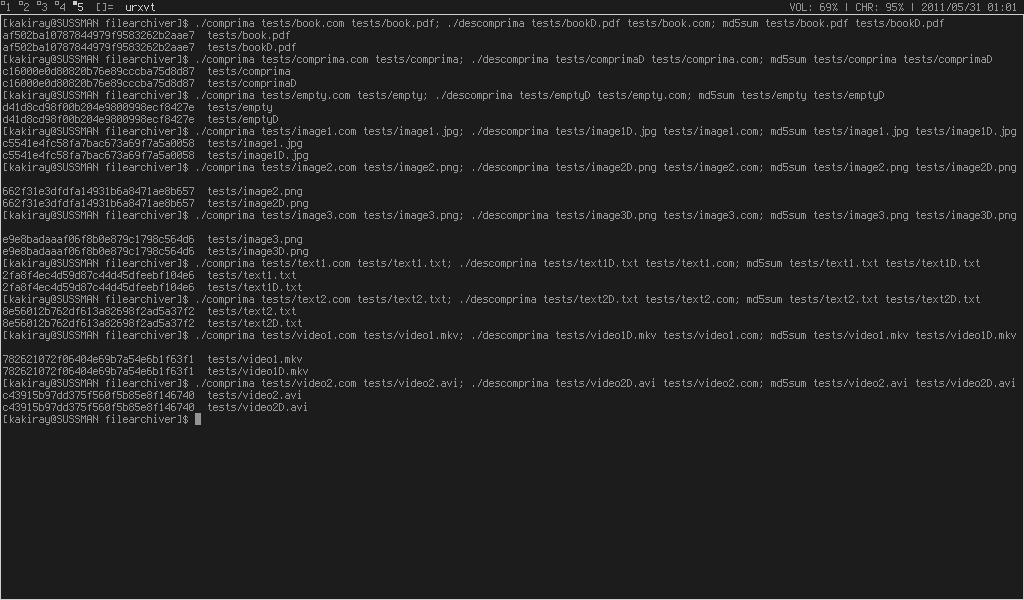
\includegraphics[width=6.2in]{testMD5.png}

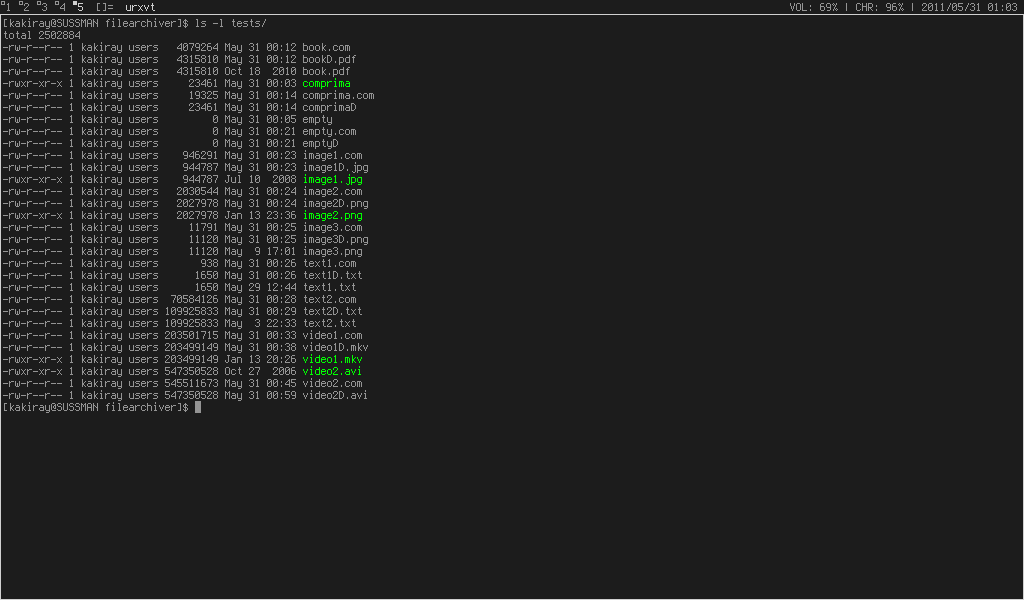
\includegraphics[width=6.2in]{testSize.png}
\end{center}

\section{Conclusão}
Em arquivos muito grandes o numero de símbolos são quase sempre chega a 256 que torna $n$ irrelevante logo programa é limitado apenas pelo tamanho da entrada. Em alguns arquivos a compressão resultou em um arquivo de tamanho maior que o original. Esses arquivos já tiveram alguma forma de compressão aplicadas a eles. Para verificar essa hipótese eu testei comprimir um arquivo anteriormente comprimido e ele também acabou tendo um tamanho maior que o original. A implementação ocorreu sem muitos problemas alem do occasional segmentation fault.

\section{Referencias}
\begin{itemize} 
\item Cormen T., Leiserson C., Rivest R., Stein C., Introduction to Algorithms 3rd Edition 2009.
\item Case S. \url{http://www.programmersheaven.com/download/2253/0/ZipView.aspx}. 1991.
\item \url{http://en.wikipedia.org/Huffman_coding}
\end{itemize}

\end{document}
